\vspace{-3mm}
\section{Methods}

Similar to state-of-the-art methodology used for polyphonic transcription~\cite{hawthorne2021sequence}, 
our approach to melody transcription involves training Transformer models~\cite{vaswani2017attention} to predict notes from audio features. 
However, to address the unique challenges of melody transcription, our approach differs in two distinct ways. 
First, because melody transcription involves operating on broad audio, we leverage representations from pre-trained models as drop-in replacements for the handcrafted spectrogram features used as inputs to other transcription systems. 
Secondly, because alignments in our dataset are approximate, we propose a new strategy for training transcription models under such conditions.

\subsection{Pre-trained representations}
\label{sec:representations}

We explore representations from two different pre-trained models for use as input features to transcription models.
In~\cite{castellon2021calm}, Castellon~et~al.\ demonstrate that representations from \jukebox~\cite{dhariwal2020jukebox}---a generative model of music audio pre-trained on $1$M songs---constitute effective features for many MIR tasks, though notably they do not experiment on transcription. 
We adopt their approach to extract features from \jukebox{} (${f_k \approx 345}$~Hz,~${d = 4800}$), though we use a deeper layer~($53$) than their default~($36$) which improved transcription performance in our initial experiments. 

We also explore features from \mtthree~\cite{gardner2021mt3}, an encoder-decoder transcription model pre-trained on a multitude of different transcription tasks (though not melody transcription). 
For this model, we use the encoder's outputs as features (${f_k = 125}$~Hz,~${d = 512}$). 
The two models have different trade-offs with respect to our setting: \jukebox{} was pre-trained on audio similar to that found in our dataset but in a generative fashion, 
whereas \mtthree{} is pre-trained on transcription but for different audio domains.

\subsection{Refined Alignments}
\label{sec:align}

\begin{figure}
    \centering
    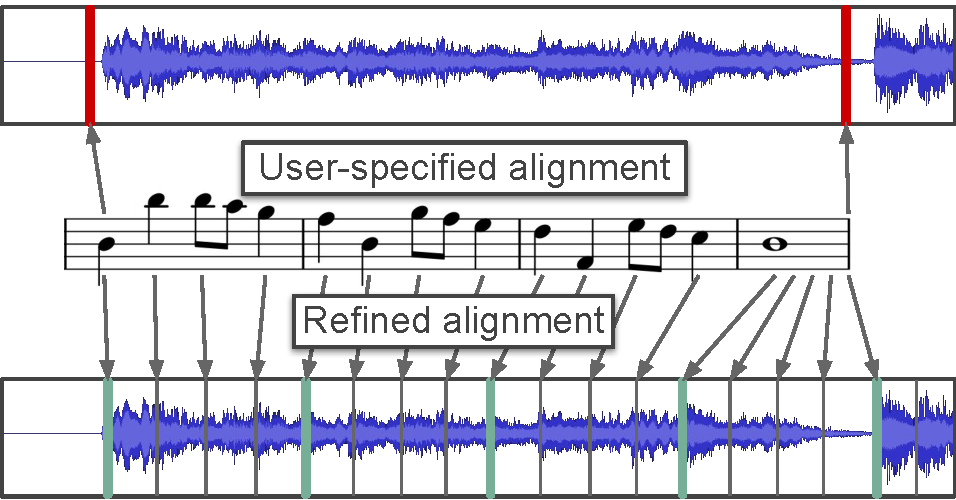
\includegraphics[width=8.1cm]{figs/alignment.pdf}
    \caption{We refine the crude user-specified alignments from \hooktheory{} by using beat and downbeat tracking. The first segment beat is mapped to the detected downbeat nearest to the user-specified starting timestamp, and remaining beats are mapped to subsequent detected beats.}
 \label{fig:alignment}
 \vspace{-5mm}
\end{figure}

The alignments between audio and HookTheory annotations are crude---users provide only an approximate starting and ending timestamp of their annotated segment within the audio. 
Because transcription methodology generally depends on precise alignments, we make an effort to refine the user-specified ones. 
To this end, we make use of the beat and downbeat detection algorithm from \madmom{}~\cite{bock2016joint,bock2016madmom}. 
Specifically, our approach aligns the first beat of the segment to the detected downbeat which is nearest to the user-specified starting timestamp. 
Then, we align the remaining beats to the subsequent detected beats (see~\Cref{fig:alignment} for an example). 
This provides a beat-level alignment for the entire segment, which we linearly interpolate to fractional subdivisions of the beat. 
Formally, we construct an alignment function $\texttt{Align} : [0,B) \to [0,T)$ that assigns each of $B$ beats in the metrical structure to a time $t \in [0,T)$ in the audio.
In an informal listening test, this produced an improved alignment for $95$ of $100$ segments, 
where the primary failure mode in the remaining $5$ segments occurred when \madmom{} detected the wrong beat as the downbeat. 
We use these refined alignments for training and evaluation and release them alongside the dataset.

\subsection{\Beatpooling}
\label{sec:beatpool}

Here we outline our approach for training transcription models in the presence of imprecise alignments. 
Existing transcription methods were largely designed for domains where perfect alignments are readily available, e.g.,~piano transcription data captured by a Disklavier. 
Despite our best efforts, the refined \hooktheory{} alignments are still imprecise when compared to alignments in the datasets used to develop existing methods. 
Consequently, in initial experiments, we found that naively adopting existing methods (specifically, \cite{hawthorne2017onsets,hawthorne2021sequence}) resulted in poor performance on our dataset and task. 
Additionally, initial experiments on training models with an alignment-free approach~\cite{graves2006connectionist} also resulted in poor performance.
% Hence, we designed a new approach to sidestep small alignment deviations.

Accordingly, to sidestep small alignment deviations, we perform a \beatpooling{} of audio features $\bm{X}~\in~\mathbb{R}^{Tf_k \times d}$ to yield features that are uniformly spaced in subdivisions of the beat (using $\texttt{Align}$---see \Cref{sec:align}) rather than in time. 
For an audio recording with $B$ beats, we sample features $\tilde{\bm{X}} \in \mathbb{R}^{4B \times d}$ at sixteenth-note intervals. 
% NOTE: Sixteenth note timestamps are obtained by linear interpolation on the madmom-detected beats
The value $\tilde{\bm{X}}_i$ is constructed by averaging all feature vectors in $\bm{X}$ that are nearest to the $i$'th sixteenth note into a single vector which acts as a proxy feature. 
For example, if a recording has a tempo of $120$~BPM, a sixteenth note represents $125$~ms of time, which would entail averaging across 
$43$ feature vectors from \jukebox{} (${f_k \approx 345}$ Hz). 
The intuition is that, while our alignments may not be precise enough to identify which of those $43$ frames contains an onset, we can be reasonably confident that it occurs \emph{somewhere} within them, and thus the relevant frame will be incorporated into the proxy. 
A similar approach was previously explored for song structure analysis in~\cite{mcfee2014analyzing}.%---here we use it for transcription. 

%Formally, given a segment of length $B$ beats or $T$ seconds and an alignment function ${a: [1, B] \mapsto [0, T]}$, \beatpooling{} yields ${\hat{\bm{X}} = \hat{\bm{x}}_1, \ldots, \hat{\bm{x}}_{4B}}$, where ${\hat{\bm{x}}_i \in \mathbb{R}^d}$, and
% \begin{gather*}
% \bm{\hat{x}}_i = \frac{1}{r_i - l_i} \sum_{j = l_i}^{r_i - 1} \bm{x}_j, \text{where} \\
% l_i = \left\lfloor a \left(\frac{2i + 5}{8} \right) \cdot f_k \right\rfloor, \text{and}~
% r_i = \left\lfloor a \left(\frac{2i + 7}{8} \right) \cdot f_k \right\rfloor.
% \end{gather*}

%\vspace{-3mm}
\subsection{Modeling}
\label{sec:modeling}

Together with the \beatpooling{} ${\tilde{\bm{X}} \in \mathbb{R}^{4B\times d}}$, we convert 
the sparse task labels ${\bm{y} \in (\mathbb{R}^+ \times \mathbb{V})^N}$ into 
a dense sequence  
${\tilde{\bm{y}} \in \{\{\varnothing\}\cup\mathbb{V}\}^{4B}}$,
which indicates whether or not an onset occurs at each sixteenth note.\footnote{This requires quantizing labels to the nearest sixteenth note. In practice, less than $1\%$ of notes in our dataset are affected by this quantization.} Formally, 
\[
\tilde{\bm{y}}_i =
\begin{cases}
n_j & \text{ if $\texttt{Align}(\frac{i}{4}) = t_j$ for some note $\bm{y}_j$}, \\
\varnothing & \text{ otherwise}.
\end{cases}
\]
We formulate melody transcription as an aligned sequence-to-sequence modeling problem and 
% attempt to estimate $p(\tilde{\bm{y}}|\tilde{\bm{X}})$. Specifically, we seek to minimize the cross-entropy loss between a parameterized family of models $p_\theta(\tilde{\bm{y}}|\tilde{\bm{X}})$ and the label distribution $p(\tilde{\bm{y}}|\tilde{\bm{X}})$.
% %using a standard cross entropy loss.
% We make a common conditional independence modeling assumption: ${p(\tilde {\bm{y}}|\tilde{\bm{X}}) = \prod_{i=0}^{4B-1} p(\tilde{\bm{y}}_i|\tilde{\bm{X}})}$.
% \pl{this is true, but is this going to freak people out who are not used to thinking about deep nets,
% which actually allow you to condition on x in a pretty extensive way? if we're worried, could emphasize this point}\john{I'm not too concerned: let's punt on this?}
attempt to predict the sequence $\tilde{\bm{y}}$ given $\tilde{\bm{X}}$. Specifically, we train models of the form ${f_{\theta} : \mathbb{R}^{4B \times d} \to \mathbb{R}^{4B \times (|\mathbb{V}| + 1)}}$, which parameterize probability distributions  ${p_\theta(\tilde{\bm{y}}_i|\bm{\tilde{X}}) = \texttt{SoftMax}(f_{\theta}(\tilde{\bm{X}})_i)}$ over elements of the sequence $\tilde{\bm{y}}$.
One unique aspect of our dataset is that absolute octave information is absent (see \Cref{sec:dataset}). 
Hence, we construct an octave-tolerant cross-entropy loss by 
identifying the octave shift amount that minimizes the standard cross-entropy loss (denoted \texttt{CE}) when applied to the labels:
\begin{equation*}
\operatorname*{min}_{\sigma \in \mathbb{Z}} \sum_{i=0}^{4B-1} \texttt{CE}(p_\theta(\tilde{\bm{y}}_i|\bm{\tilde{X}}), \texttt{OctaveShift}(\tilde{\bm{y}}_i, \sigma)).
\end{equation*}

We require a thresholding scheme to convert the dense sequence of soft probability estimates $p_\theta(\tilde{\bm{y}}_i|\tilde{\bm{X}})$ into a sparse sequence of notes required by our task (see \Cref{sec:task}). Given a threshold $\tau\in\mathbb{R}$ (in practice, tuned on validation data), we define a sorted \emph{onset list}
\[
\mathcal{I} = \texttt{Sort}(\{i \in \{0,\dots,4B-1\} : p_\theta(\tilde{\bm{y}}_i = \varnothing|\tilde{\bm{X}}) < \tau\}).
\]
This should be interpreted as a list of $N$ metrical positions where an onset likely occurs. The timings of these onsets are given by the alignment, and we will predict the note-value with the highest probability. The sparse melody transcription is thus defined for $j=1,\dots,N$ by
\begin{align*}
&\texttt{Transcribe}(\tilde{\bm{X}})_j = (t_j,n_j),\text{ where }\\
&\quad t_j = \texttt{Align}\left(\frac{\mathcal{I}_j}{4}\right),\\
&\quad n_j = \argmax_{v\in\mathbb{V}} p_\theta(\tilde{\bm{y}}_{\mathcal{I}_j} = v|\tilde{\bm{X}}).
\end{align*}